% !TeX document-id = {c68ea1ac-ebac-4541-a297-17005c6d2297}
% !TeX encoding = UTF-8
% !TeX spellcheck = en_US
% !TeX TS-program = pdflatex
% !TeX TXS-program:bibliography = biber -l zh__pinyin --output-safechars %

\documentclass[aspectratio=169,10pt
%	,handout
	,noamsthm
]{beamer}

% to be `\input` in subfolders,
% ... therefore the path should be relative to subfolders.

\usepackage{iftex}
\ifPDFTeX
\else
	\usepackage[UTF8
		,heading=false
		,scheme=plain % English Document
	]{ctex}
\fi
%\ctexset{autoindent=true}
\usepackage{indentfirst}

\input{../.modules/basics/macros.tex}
\input{../.modules/preamble_base.tex}
\input{../.modules/preamble_beamer.tex}
\input{../.modules/basics/biblatex.tex}


%Misc
	\usepackage{lilyglyphs}
	\newcommand{\indicator}{$\text{\clefG}$}
	\newcommand{\indicatorInline}{$\text{\clefGInline}$}

\newcommand{\legacyReference}{{
%	\clearpage\par
%	\quad\clearpage
	\def{\midquote}{\textbf{PAST WORK, AS TEMPLATE}}
	\newparagraph
}}

% Settings
\counterwithout{equation}{section}
\mathtoolsset{showonlyrefs=false}
%\DeclareTextFontCommand{\textbf}{\sffamily}

% Spacing
\geometry{footnotesep=2\baselineskip} % pre footnote split
\setlength{\parskip}{.5\baselineskip}
\renewcommand{\baselinestretch}{1.15}


%% List
%	\setlist*{
%		listparindent=\parindent
%		,labelindent=\parindent
%		,parsep=\parskip
%		,itemsep=1.2\parskip
%	}


\addtobeamertemplate{navigation symbols}{}{%
    \usebeamerfont{footline}%
%    \usebeamercolor[fg]{footline}%
    \hspace{1em}%
    \large\insertframenumber/\inserttotalframenumber
}

\makeatletter
\setbeamertemplate{headline}
{%
    \begin{beamercolorbox}[wd=\paperwidth,colsep=1.5pt]{upper separation line head}
    \end{beamercolorbox}
    \begin{beamercolorbox}[wd=\paperwidth,ht=2.5ex,dp=1.125ex,%
      leftskip=.3cm,rightskip=.3cm plus1fil]{title in head/foot}
      \usebeamerfont{title in head/foot}\insertshorttitle
    \end{beamercolorbox}
    \begin{beamercolorbox}[wd=\paperwidth,ht=2.5ex,dp=1.125ex,%
      leftskip=.3cm,rightskip=.3cm plus1fil]{section in head/foot}
      \usebeamerfont{section in head/foot}%
      \ifbeamer@tree@showhooks
        \setbox\beamer@tempbox=\hbox{\insertsectionhead}%
        \ifdim\wd\beamer@tempbox>1pt%
          \hskip2pt\raise1.9pt\hbox{\vrule width0.4pt height1.875ex\vrule width 5pt height0.4pt}%
          \hskip1pt%
        \fi%
      \else%  
        \hskip6pt%
      \fi%
      \insertsectionhead
    \end{beamercolorbox}
% Code for subsections removed here
}
\makeatother

\usepackage{tikz}
%\usepackage{snapshot}

%Title
	\title{Understanding Holographic Entanglement}
	\subtitle{With gravitational path integral \& tensor network}
	\author{\textkai{赖文昕} \texttt{2019311369}}
	\institute{\large\ccbyncsajp}
	\date{}


\newcommand{\veccol}[1]{\pqty{
	\begin{smallmatrix}
		#1
	\end{smallmatrix}
}}

\addbibresource{holography.bib}
%\usepackage{cprotect}

\usepackage{cancel}
\newcommand{\slot}{{\,\bullet}}

\begin{document}
{%%% TITLEPAGE
\setbeamercolor{title in head/foot}{
		use=palette quaternary
		,fg=palette quaternary.bg
	}
\logo{}
\begin{frame}
	\titlegraphic{\vspace{2\baselineskip}}
	\titlepage
	\tikz [remember picture,overlay]
	\node at ([
		yshift=-3.2\baselineskip,xshift=.2\linewidth
	] current page.center) {
		\begin{minipage}{.6\textwidth}
		\flushright
		
\includegraphics[height=.45\textheight]{img/escher.jpg}
		\quad
		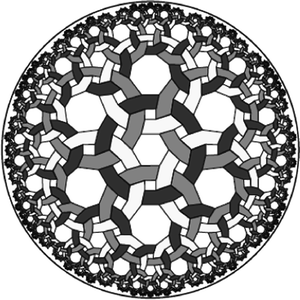
\includegraphics[height=.45\textheight]{img/escher_links.png}
		\\[1ex]
		\footnotesize\textcite{Dunham:Escher} on Escher's art
		\hspace{0em}
		\end{minipage}
	};

\end{frame}
}%%% TITLEPAGE


\begin{frame}{Introduction}
\begin{itemize}
\item \textbf{Question:} how can we \textit{``prepare'' / construct a state,} e.g.
	\begin{itemize}
	\item vacuum: $\rho = \dyad{0}$
	\item thermal: $\rho \propto \sum_n e^{-\beta H} \dyad{n}$
	\end{itemize}
	... in a \textit{holographic} system? \\
\pause
\item \textbf{Answer:} via holography! (\textit{duh...})
	\begin{itemize}
	\item Gravitational path integral\pause
	\item Tensor network
	\end{itemize}\pause
\item Entanglement entropy captures some ``structure'' of the state
\end{itemize}
\end{frame}


\section{Review: boundary entanglement as gravitational saddles}


\begin{frame}{Recall: Path Integral in the Boundary \& the Bulk}{%
	\textcite{Lewkowycz:2013nqa}:\,\citetitle{Lewkowycz:2013nqa}%
}
	\begin{columns}
	\begin{column}{.3\textwidth}
		\begin{figure}[!h]
		\centering
		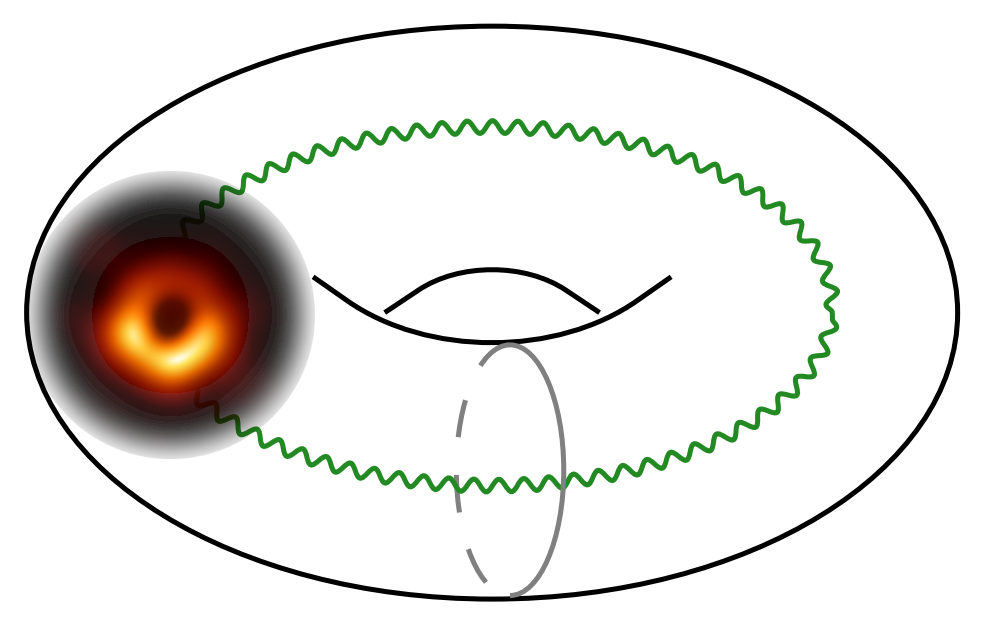
\includegraphics[width=\linewidth]{img/blackhole_donut.png}
		\caption{Thermal $\mcal{Z}_\beta$}
		
		\footnotesize
		Thermal partition function \\ in the bulk \& the boundary
		\\[2ex]
		\scriptsize
		Image made from \textcite{Benjamin:2020mfz} and the EHT black hole photo
		\end{figure}
	\end{column}
	\begin{column}{.7\textwidth}
		\begin{itemize}
		\item In \textit{any} field theory, a thermal state\\ can be prepared by a path integral;
		\item In a \textit{holographic} theory, $
			\mcal{Z}_{\pd B} = \mcal{Z}_{B\textit{ulk}}
		$,\\
		a boundary state can be prepared by a bulk path integral.
	\pause
		\begin{itemize}
		\item e.g.~the thermo-field double $\leftrightarrow$ the BTZ black hole\\
			Note that the Euclidean BTZ geometry is smooth:\\
			filling in the $t_E$ cycle (\textit{not} the $\phi$ cycle) of the torus
		
		\item c.f.~Chern-Simons/WZW: not quite the same
		\end{itemize}
		\end{itemize}
	\end{column}
	\end{columns}
\end{frame}


\begin{frame}{Recall: Gravitational Path Integral}{%
	\textcite{Lewkowycz:2013nqa}:\,\citetitle{Lewkowycz:2013nqa}%
}
	\begin{columns}
	\begin{column}{.3\textwidth}
		\begin{figure}[!h]
		\centering
		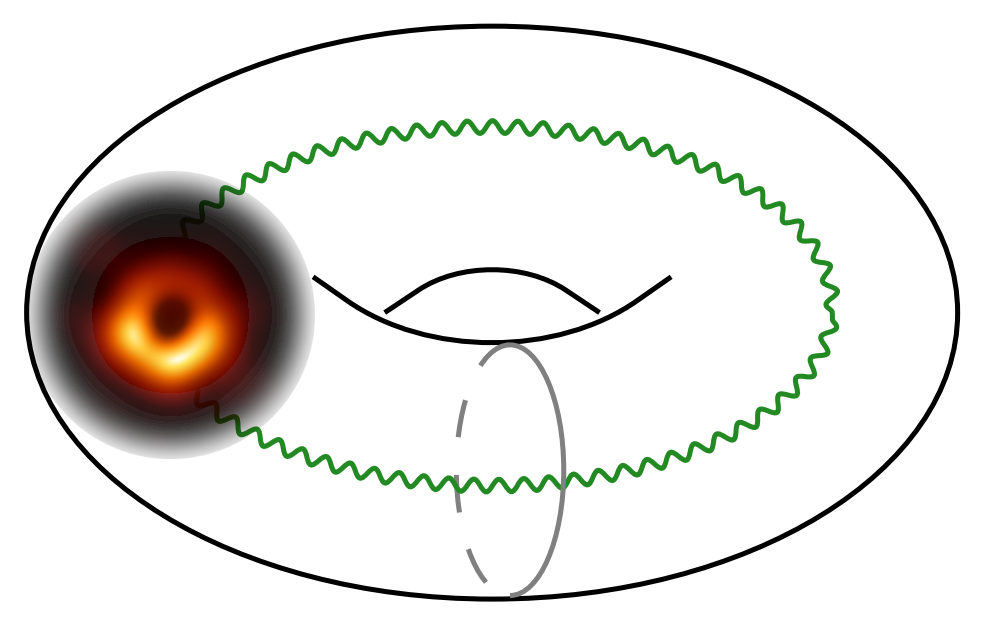
\includegraphics[width=\linewidth]{img/blackhole_donut.png}
		\caption{Thermal $\mcal{Z}_\beta$}
		
		\footnotesize
		Thermal partition function \\ in the bulk \& the boundary
		\\[2ex]
		\scriptsize
		Image made from \textcite{Benjamin:2020mfz} and the EHT black hole photo
		\end{figure}
	\end{column}
	\begin{column}{.7\textwidth}
		\begin{equation}
			\mcal{Z}_{\pd B} = \mcal{Z}_{B\textit{ulk}}
		\end{equation}
		\vspace{-1.2\baselineskip}
		\begin{itemize}
		\item Replica trick: entanglement entropy for a region $R$:
		\begin{equation}
			S_R
			= \Tr
				\rho_R \log \rho_R
			\ \Leftarrow\ %
			\Tr \rho_R^n \equiv \mcal{Z}_n
		\end{equation}
		i.e.~reduced to the partition function of the $n$-replica.\\
		It can be deployed in the boundary \& the bulk!
			\begin{itemize}
			\item Boundary: static geometry, but the field theory is usually strongly coupled --- often difficult!
		\pause
			\item Bulk: dynamic geometry, weakly coupled gravity:\\
			gravity fills in the bulk smoothly, \\
			$
				\mcal{Z} \sim \sum_i e^{-S_i[g_{\mu\nu}]}
			$: sum over classical saddles
			\end{itemize}
		\end{itemize}
	\end{column}
	\end{columns}
\end{frame}


\begin{frame}{Recall: Replica Trick and the Ryu--Takayanagi Proposal}{%
	\textcite{Lewkowycz:2013nqa}:\,\citetitle{Lewkowycz:2013nqa}%
}
	\begin{columns}
	\begin{column}{.425\textwidth}
		\begin{figure}[!h]
		\centering
		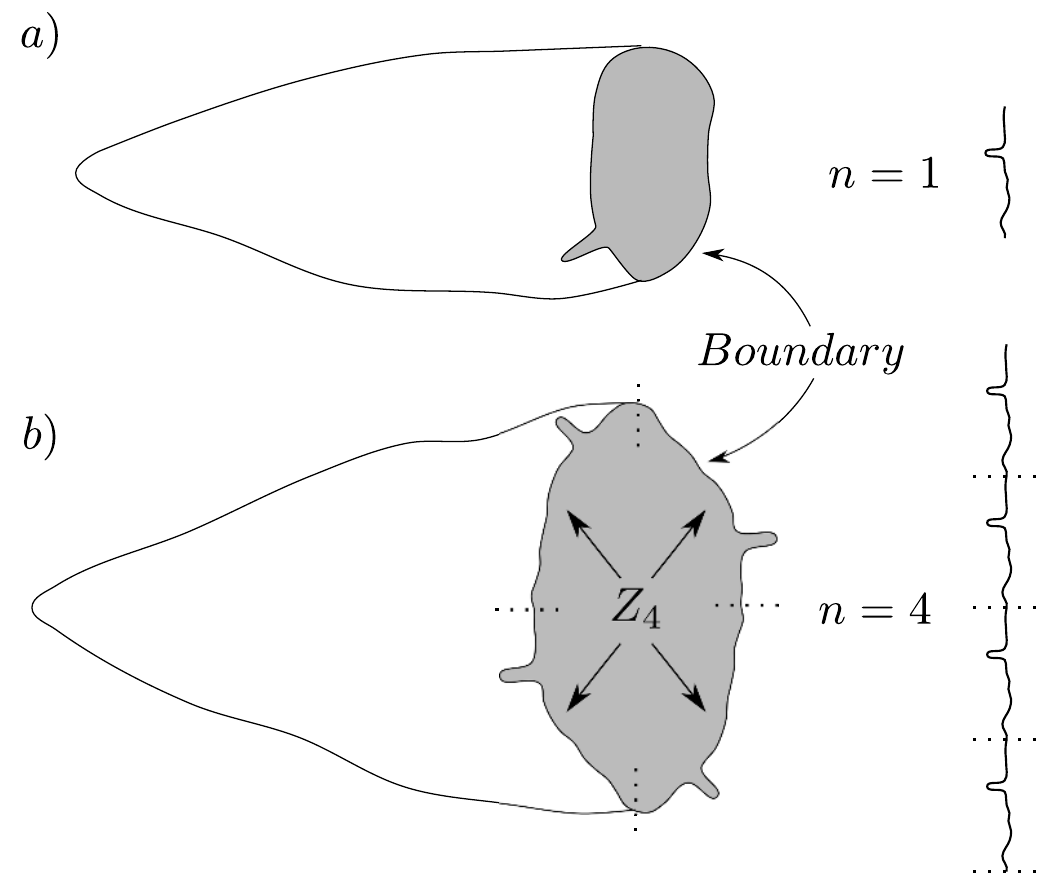
\includegraphics[width=\linewidth]{img/replica.png}
		\caption{The bulk replica \cite{Lewkowycz:2013nqa}}
		\end{figure}
	\end{column}
	\begin{column}{.55\textwidth}
		\begin{itemize}
		\item $\mcal{Z} \sim \sum_i e^{-S_i[g_{\mu\nu}]}$, saddle pt.\ approx.\\
			$\To$ minimize $S[g_{\mu\nu}]$ on the $n$-replica $\widetilde{\mcal{M}}_n$
		\item $\widetilde{\mcal{M}}_n/\mbb{Z}_n$: conical singularity at the $\mbb{Z}_n$; $n\to 1$,\\
			$\To$ minimize the area of the $\mbb{Z}_n$ fixed point\\
			$\To$ the extremal surface, the RT surface
		\\[2ex]
	\pause
		\item \textbf{Lesson:} use bulk path integral to:
			\begin{itemize}
			\item prepare the states
			\vspace{-1ex}
			\item compute the entanglement entropy
			\end{itemize}
			This requires holography, \\
			but not necessarily $\mrm{AdS/CFT}$!
		\end{itemize}
	\end{column}
	\end{columns}
\end{frame}


\section{Compare: bulk emergence from tensor networks}


\begin{frame}{Prepare states via Tensor Networks}{%
	\textcite{Vidal:2007hda}, \textcite{Swingle:2009bg}. Reviewed by \textcite{Rangamani:2016dms}.
}
	\begin{columns}
	\begin{column}{.4\textwidth}
		\begin{figure}[!h]
		\centering
		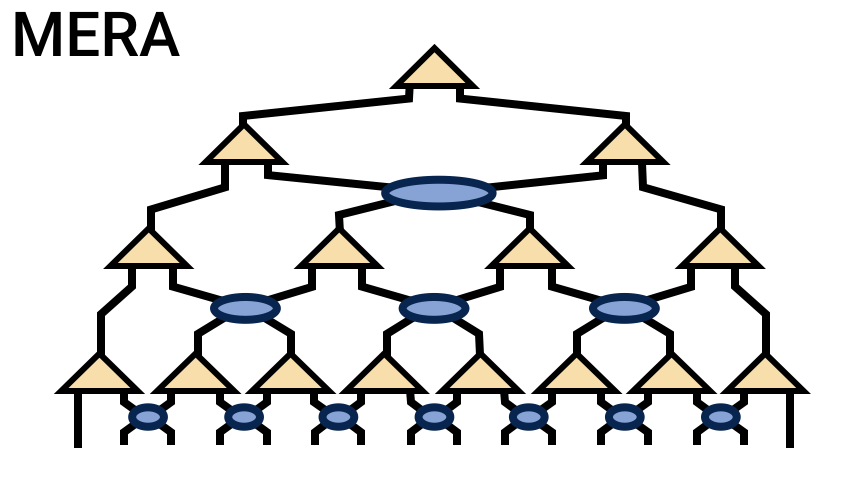
\includegraphics[width=\textwidth]{img/MERA.png}
		\caption{MERA}
		
		\small
		Multi-scale Entanglement\\
		Renormalization Ansatz
		\\[2ex]
		\footnotesize
		Image from \https{tensornetwork.org}
		\end{figure}
	\end{column}
	\begin{column}{.6\textwidth}
		\begin{itemize}
		\item Gravitational path integral: a spacetime perspective\\
		Tensor network: on a constant time slice
	\pause
		\item States constructed with tensor networks:\\
		common in condensed matter (e.g.~DMRG)\\
		\item To find the ground state of a system
			\begin{itemize}
			\item Write down a tensor network \\
			as an \textbf{ansatz} for the ground state;\\
			\item Vary the components of each tensor \\
			to achieve minimal energy --- \textbf{optimization!}
			\end{itemize}
		\end{itemize}
	\end{column}
	\end{columns}
\end{frame}


\begin{frame}{AdS Bulk as a Tensor Network}{Reviewed by \textcite{Harlow:2018fse}:\,\citetitle{Harlow:2018fse}}
	\begin{columns}
	\begin{column}{.35\textwidth}
		\begin{figure}[!h]
		\centering
		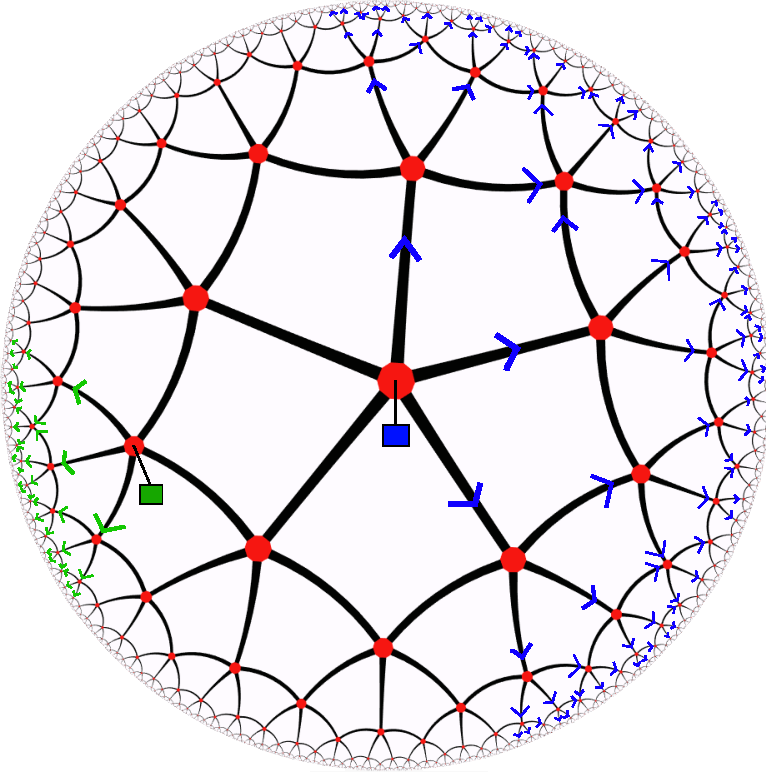
\includegraphics[height=.55\textheight]{img/pentagonpush.pdf}
		\caption{The HaPPY code \cite{Pastawski:2015qua,Harlow:2018fse}}
		\end{figure}
	\end{column}
	\begin{column}{.65\textwidth}
		\begin{itemize}
		\item Gravitational path integral: a spacetime perspective\\
		Tensor network: on a constant time slice
	\pause
		\item Dual geometry in the bulk is understood as\\ the ``continuous limit'' of a \textit{tensor network}\\
			\begin{itemize}
			\item Node: tensor acting on the Hilbert space
			\item Leg: index to be contracted
				\begin{itemize}
				\item $1\times{}$free leg \\takes in bulk local operator insertions
				\item $5\times{}$contracted leg \\propagates the bulk insertions to the boundary
				\end{itemize}
			\end{itemize}
		\end{itemize}
	\end{column}
	\end{columns}
\end{frame}


\begin{frame}{RT from the tensor network}{\textcite{Harlow:2018fse}:\,\citetitle{Harlow:2018fse}}
	\begin{columns}
	\begin{column}{.35\textwidth}
		\begin{figure}[!h]
		\centering
		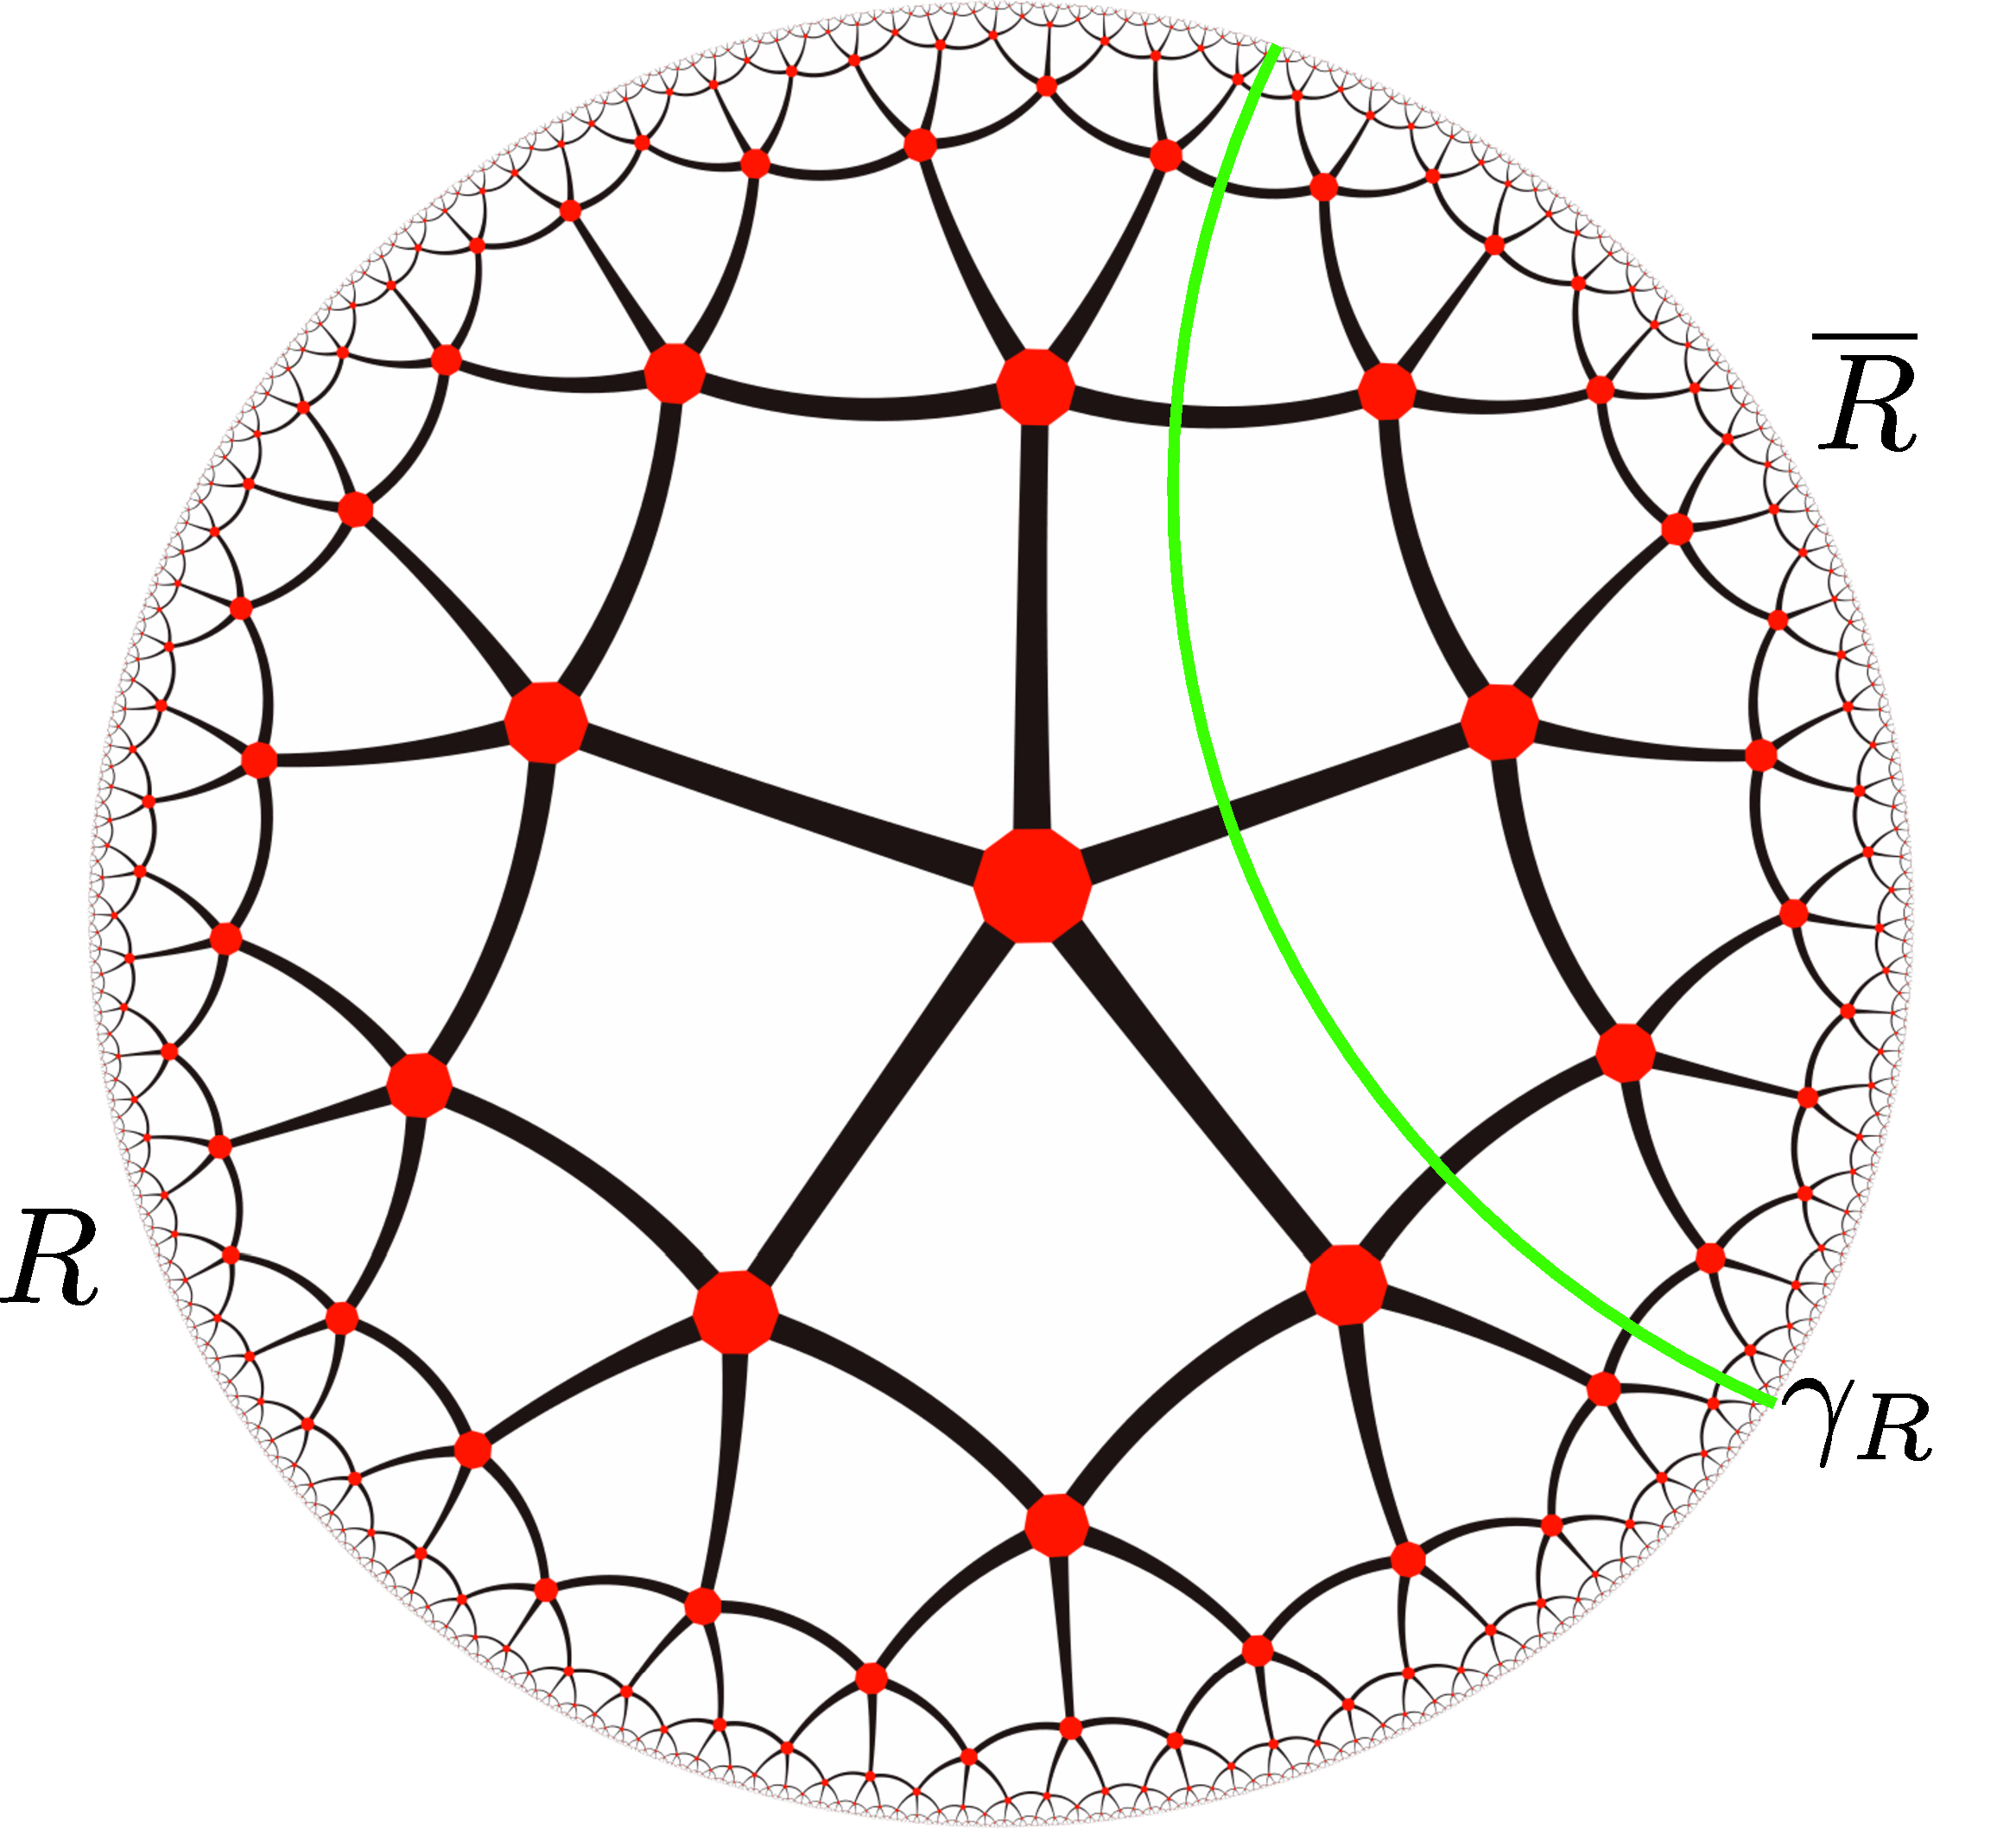
\includegraphics[height=.55\textheight]{img/cutnetwork.pdf}
		\caption{The HaPPY code \cite{Pastawski:2015qua,Harlow:2018fse}}
		\end{figure}
	\end{column}
	\begin{column}{.65\textwidth}
		\begin{itemize}
		\item ``Entanglement'' between $R$ and $\bar{R}$:\\
		$\propto$ min \# of links connecting the two regions\\
		Naturally, entropy $=$ bulk area!
	\pause
		\item ``Complexity'': \# of nodes\\
		Proposal: complexity $=$ bulk volume!\\
		{\footnotesize See e.g.~\textcite{Susskind:2014rva}}
	\pause
		\item Note: how to actually take the continuous limit?\\
		``Real time'' path integral on a constant time slice
			\begin{itemize}
			\item cMERA: \textcite{Nozaki:2012zj}
			\item ``Path-Integral Optimization'':\\
			\textcite{Boruch:2021hqs}
			\end{itemize}
		\end{itemize}
	\end{column}
	\end{columns}
\end{frame}


\begin{frame}{The Lesson}
	\begin{itemize}\large
	\item The Ryu--Takayanagi proposal: $S \sim \frac{A}{4G_N}$
		\begin{itemize}\normalsize
		\item ... seems to be universal in holographic systems, 
		\item ... where boundary states can be constructed from some sort of bulk operations:
			\begin{itemize}
			\item Gravitational path integral
			\item Tensor network
			\end{itemize}
		\end{itemize}
	\item Applications: beyond standard $\mrm{AdS}_3/\mrm{CFT}_2$
		\begin{itemize}\normalsize
		\item Cutoff holography: \textcite{Lewkowycz:2019xse}
		\vspace{-.5ex}
		\item Flat holography: \textcite{Apolo:2020bld,Apolo:2020qjm}
		\end{itemize}
	\end{itemize}
\end{frame}


\section{Application: cutoff $\mrm{AdS}_3\,/\,T\bar{T}$ deformed theory}


\begin{frame}{Cutoff $\mrm{AdS}_3\,/\,T\bar{T}$ deformed theory}{%
	\textcite{McGough:2016lol}%
}
	\begin{columns}
	\begin{column}{.35\textwidth}
		\begin{figure}[!h]
		\centering
		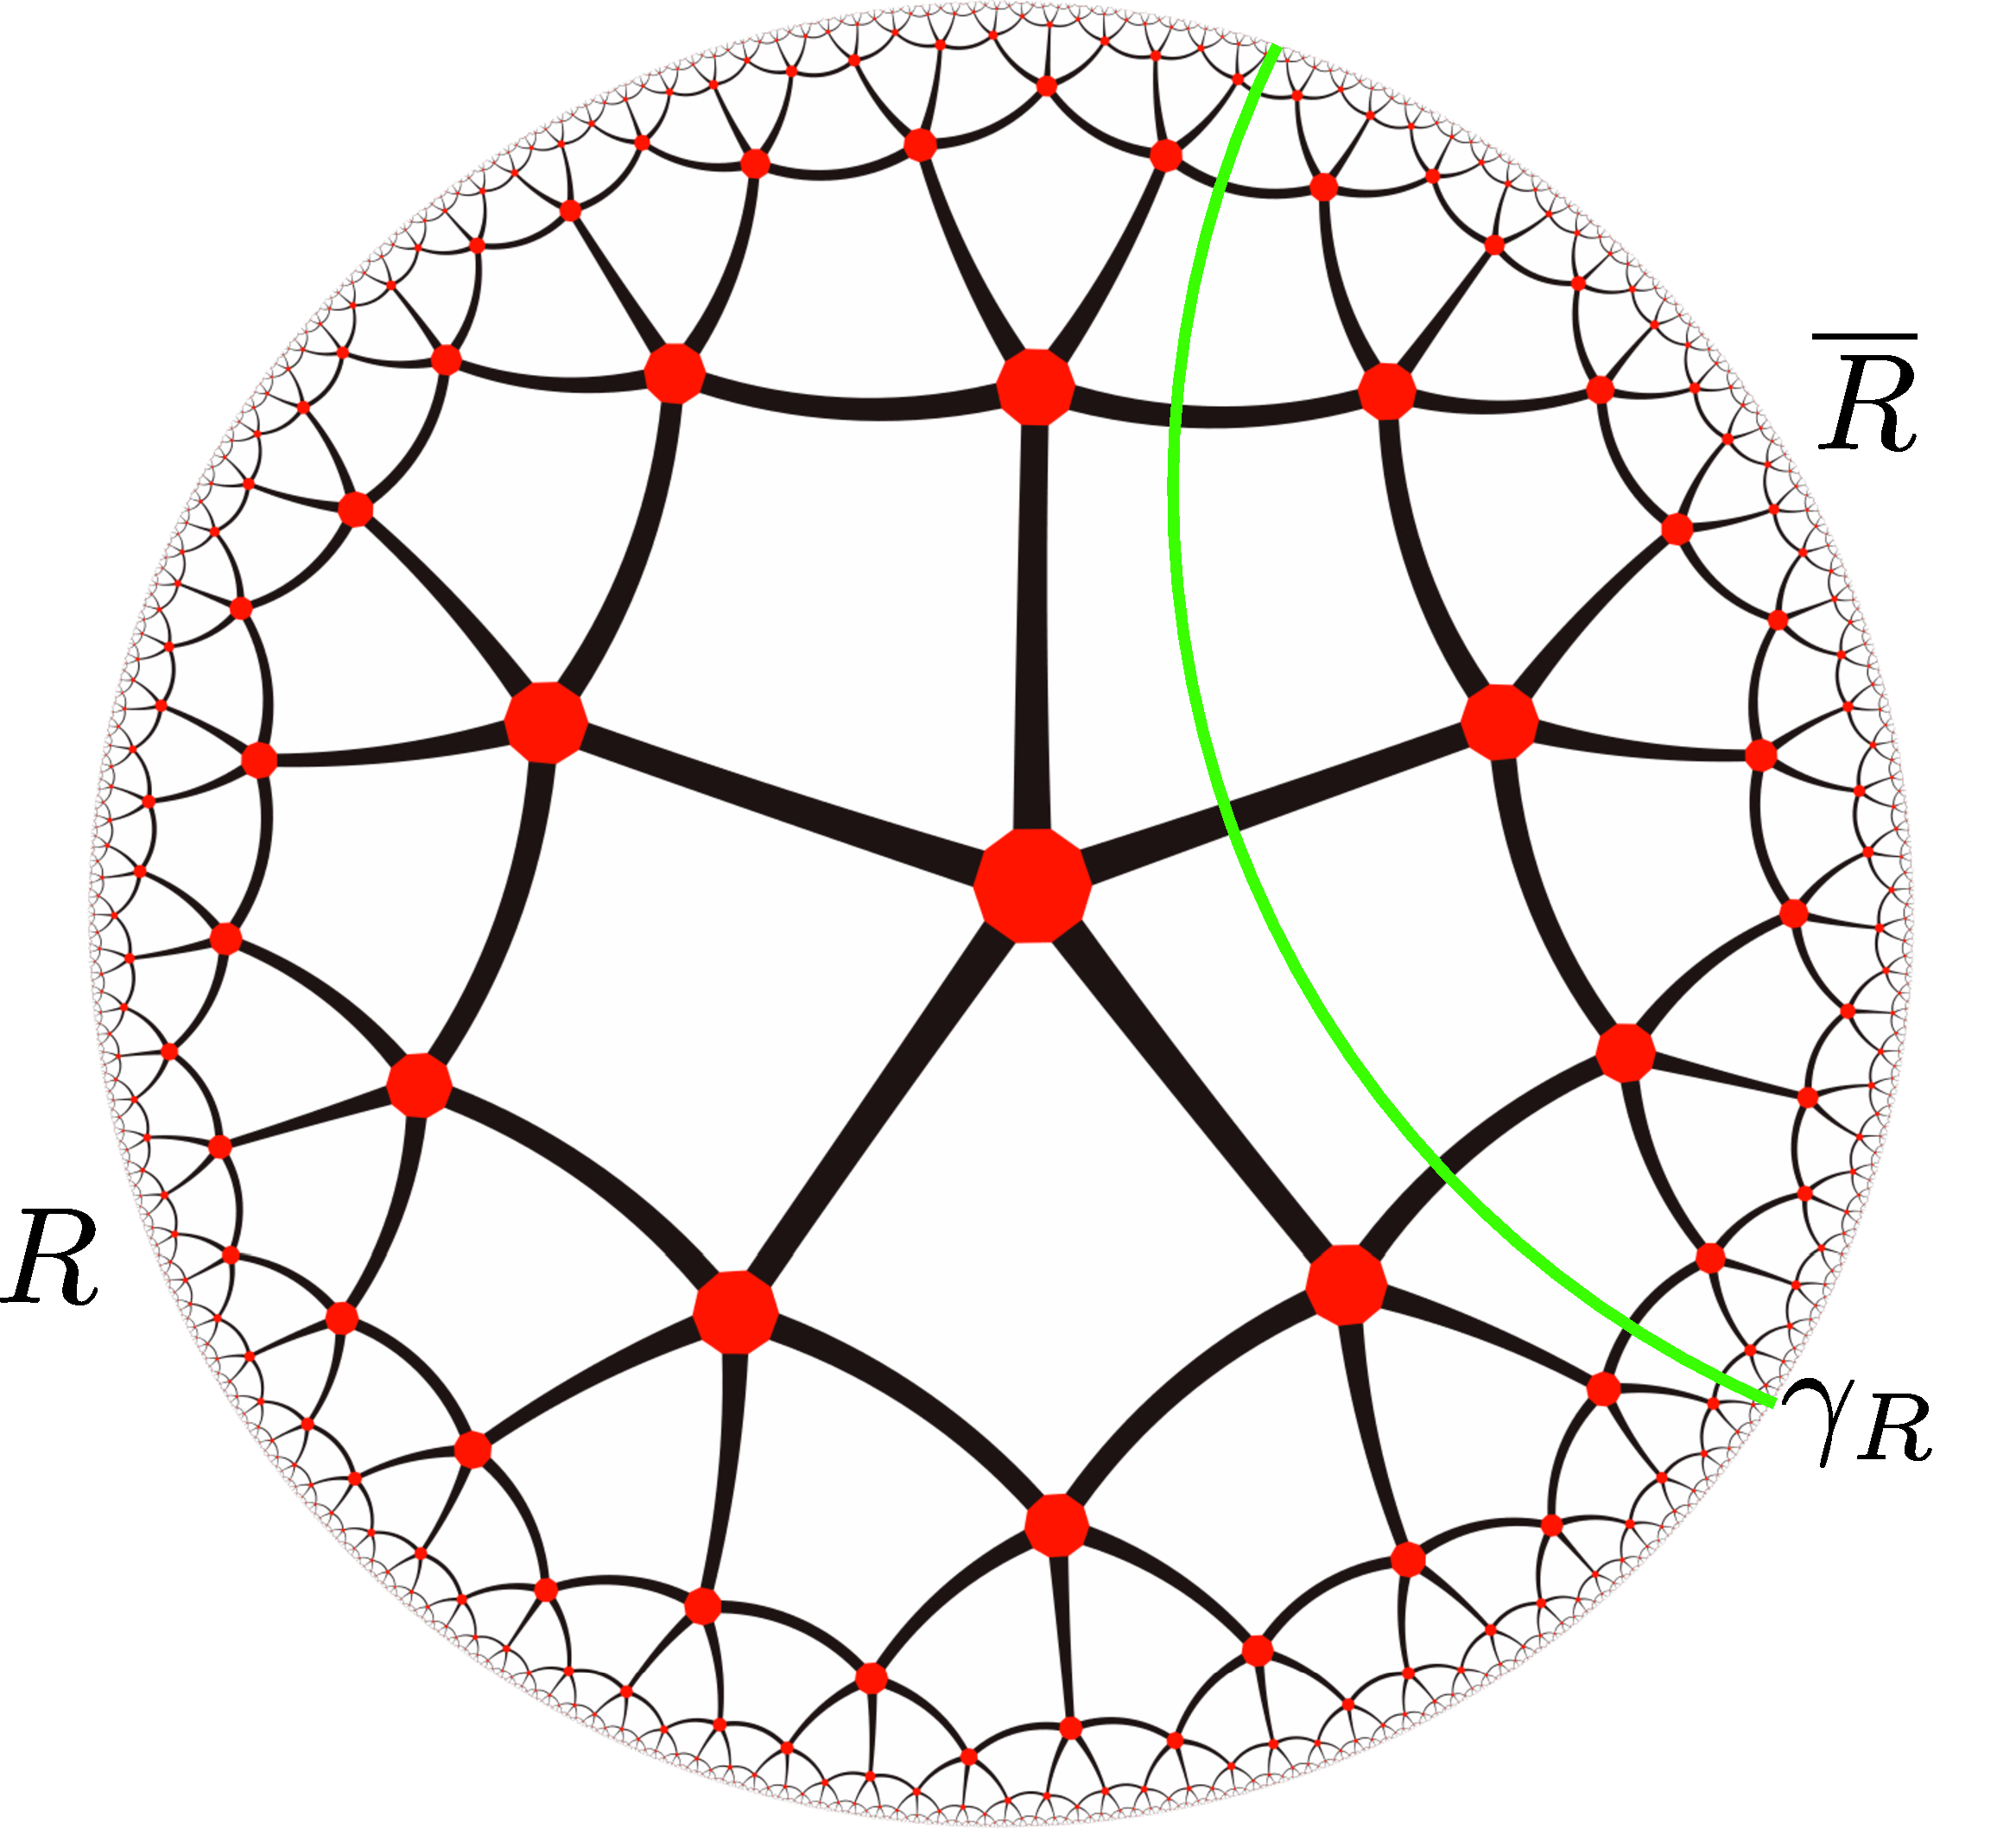
\includegraphics[height=.55\textheight]{img/cutnetwork.pdf}
		\caption{The HaPPY code \cite{Pastawski:2015qua,Harlow:2018fse}}
		\end{figure}
	\end{column}
	\begin{column}{.65\textwidth}
		\begin{itemize}
		\item $\mrm{AdS}_3$ with finite cutoff:\\
		\textit{holographic renormalization} of the boundary theory
		
	\pause
		
			\begin{itemize}
			\item This is clear in the tensor network picture\\
			``coarse-graining''
			\end{itemize}
		
	\pause
		
		\item Deform the boundary $\mrm{CFT}_2$ with some operator:\\
		$\mrm{CFT}_2^{\,(\mrm{UV})} \leadsto {}$deformed theory$^{\,(\mrm{IR})}$
		
		\item Surprisingly, we were able to find the deformed theory!\\
		$
			\var{S} \propto \mu\,(T\bar{T})_\mu,\ %
			T\bar{T}
			= \frac{1}{8} \pqty{
					T^{\alpha\beta} T_{\alpha\beta}
					- (T^\alpha_\alpha)^2
				}
		$
		
			\begin{itemize}
			
			\item See e.g.~\textcite{Smirnov:2016lqw}
			
			\item \textcite{McGough:2016lol}:\\
			\citetitle{McGough:2016lol}
			
			\end{itemize}
		
		\end{itemize}
	\end{column}
	\end{columns}
\end{frame}


\begin{frame}{Holographic Entanglement in Cutoff $\mrm{AdS}_3$}{%
	\textcite{Lewkowycz:2019xse}%
}
	\begin{columns}
	\begin{column}{.35\textwidth}
		\begin{figure}[!h]
		\centering
		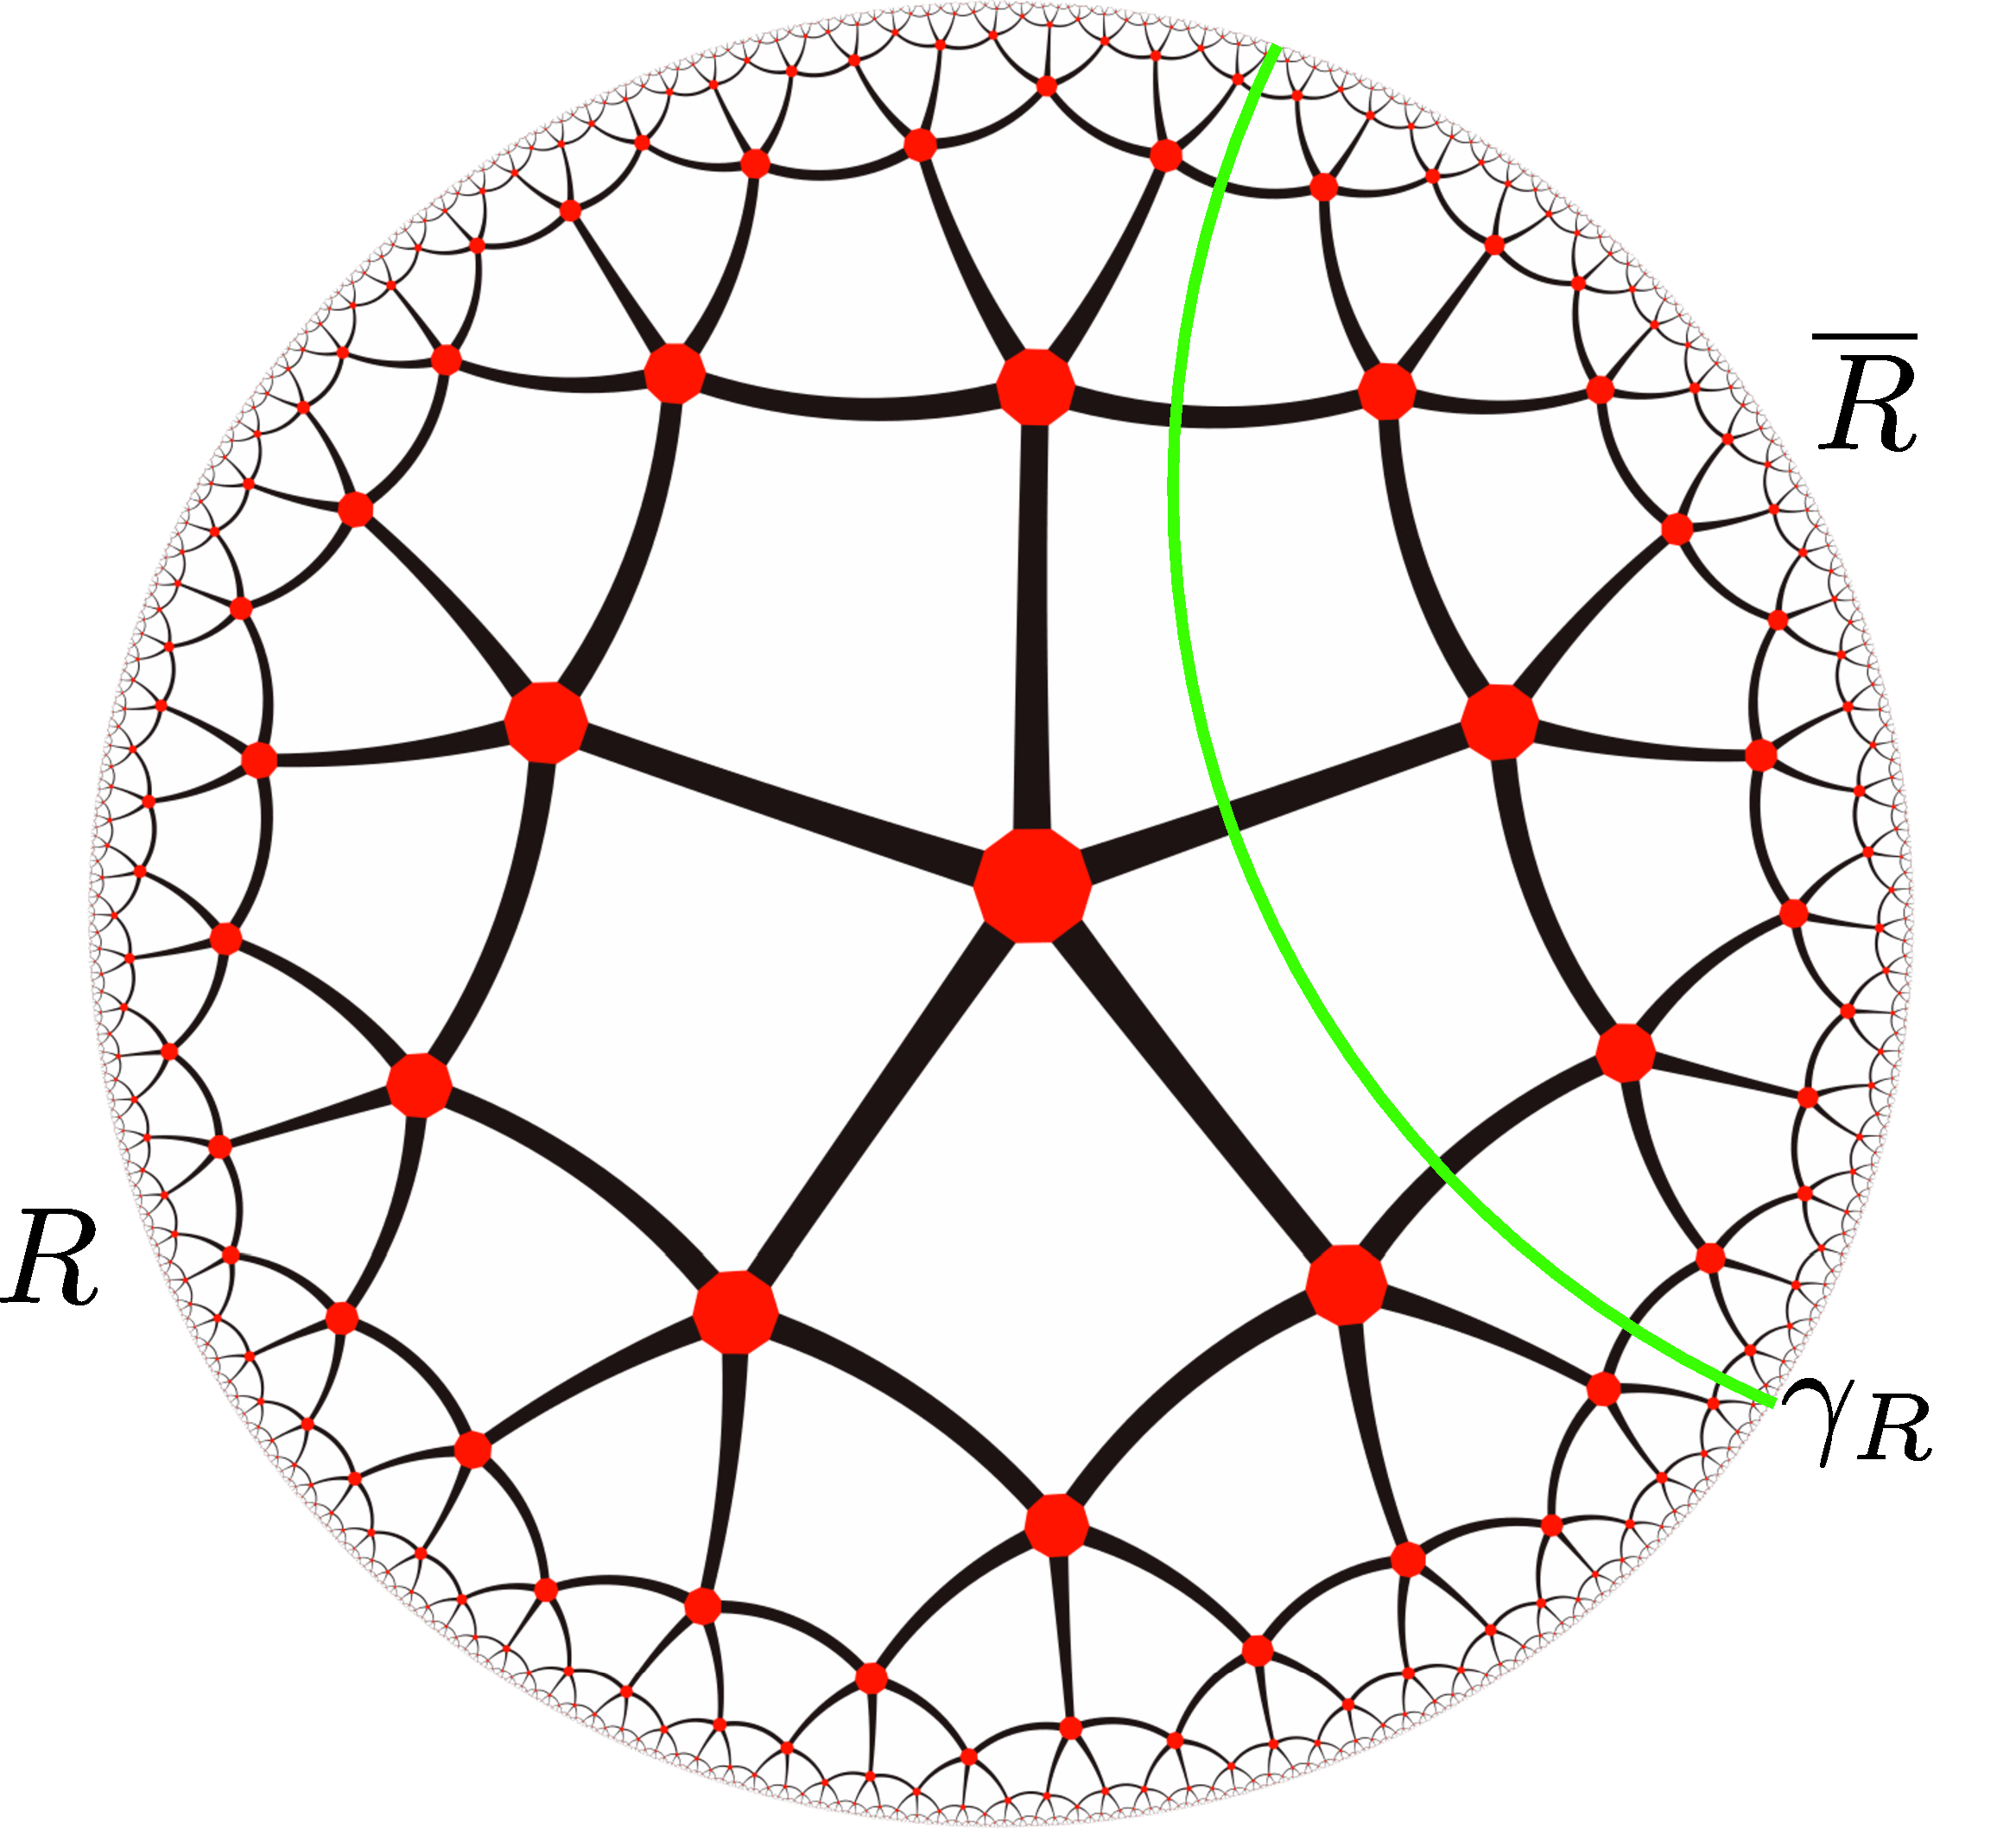
\includegraphics[height=.55\textheight]{img/cutnetwork.pdf}
		\caption{The HaPPY code \cite{Pastawski:2015qua,Harlow:2018fse}}
		\end{figure}
	\end{column}
	\begin{column}{.65\textwidth}
		\begin{itemize}
		\item If we \textit{assume} that the tensor network intuition is valid,\\
		Then the RT proposal should still hold!
		
			\begin{itemize}
			\item This is shown by \textcite{Lewkowycz:2019xse}
			\end{itemize}
		
	\pause
		
		\item Generalization of $A$ in $S \sim \frac{A}{4G_N}$:
		$A$ is actually the gravitational charge of the \textit{replica symmetry},
		
			\begin{itemize}
			\item ... \textit{analytically continued} from $\mbb{Z}_n$ to $U(1)$,
		\vspace{-.5ex}
			\item ... corresponds to the Killing horizon generator / \textit{modular flow generator} $\xi$. 
			
			\item This would in turn give us a hint of the modular flow\\
			 in the $T\bar{T}$ deformed theory! (\textit{ongoing work})
			
			\end{itemize}
		
		\end{itemize}
	\end{column}
	\end{columns}
\end{frame}


\begin{frame}{Further Reading \& Outlook}
	\begin{itemize}
	\item Single-trace $T\bar{T}$ duality and the flow towards to UV
		\begin{itemize}
		\item \fullcite{Apolo:2019zai}
		\end{itemize}
	\item Quantum error correction:
		\begin{itemize}
		\item \fullcite{Jahn:2021uqr}
		\end{itemize}
	\item Tensor network for flat spacetime?
		\begin{itemize}
		\item \fullcite{May:2016dgv}
		\end{itemize}
	\end{itemize}
\end{frame}


\begin{frame}[allowframebreaks]{References}
\renewcommand*{\bibfont}{\footnotesize}
\printbibliography[%
%	title = {参考文献} %
	,heading = bibintoc
]
\end{frame}


\end{document}
